\begin{figure}[htb]
    \centering
    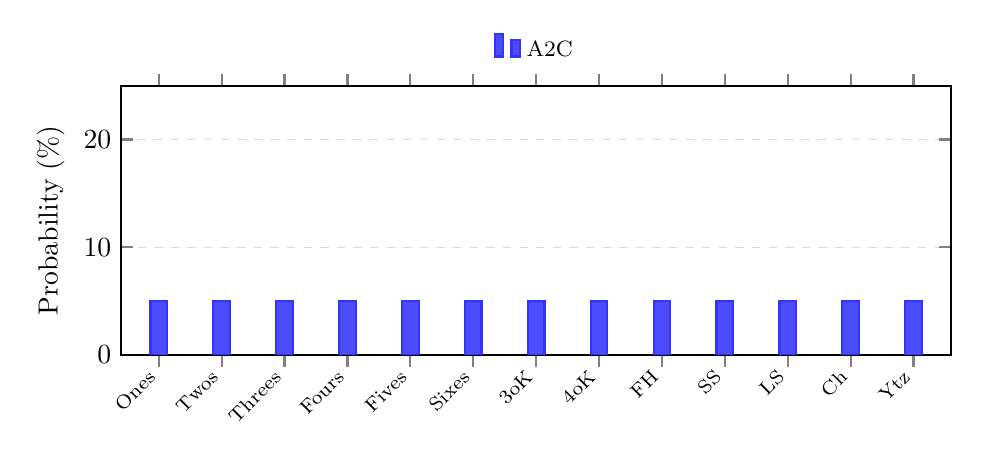
\begin{tikzpicture}
        \begin{axis}[
                ybar=1pt,
                width=\columnwidth,
                height=5cm,
                bar width=6pt,
                symbolic x coords={Ones,Twos,Threes,Fours,Fives,Sixes,3oK,4oK,FH,SS,LS,Ch,Ytz},
                xtick=data,
                xticklabel style={font=\scriptsize, rotate=45, anchor=east},
                ylabel={Probability (\%)},
                ymin=0,
                ymax=25,
                ymajorgrids=true,
                grid style={dashed,gray!30},
                legend style={
                        at={(0.5,1.05)},
                        anchor=south,
                        legend columns=3,
                        font=\footnotesize,
                        draw=none,
                        fill=none
                    },
                enlarge x limits=0.05,
                axis line style={thick},
                tick style={thick},
            ]

            % DP
            % \addplot[fill=black!70, draw=black!80, thick] coordinates {
            %         (Ones,5) (Twos,5) (Threes,5) (Fours,5) (Fives,5) (Sixes,5)
            %         (3oK,5) (4oK,5) (FH,5) (SS,5) (LS,5) (Ch,5) (Ytz,5)
            %     };

            % A2C
            \addplot[fill=blue!70!white, draw=blue!80!white, thick] coordinates {
                    (Ones,5) (Twos,5) (Threes,5) (Fours,5) (Fives,5) (Sixes,5)
                    (3oK,5) (4oK,5) (FH,5) (SS,5) (LS,5) (Ch,5) (Ytz,5)
                };

            % PPO
            % \addplot[fill=red!60!white, draw=red!80!white, thick] coordinates {
            %         (Ones,5) (Twos,5) (Threes,5) (Fours,5) (Fives,5) (Sixes,5)
            %         (3oK,5) (4oK,5) (FH,5) (SS,5) (LS,5) (Ch,5) (Ytz,5)
            %     };

            \legend{A2C}

        \end{axis}
    \end{tikzpicture}
    \caption{First category chosen distribution (placeholder data)}
    \label{fig:strategy-first-category}
\end{figure}
